\documentclass[a4paper,10pt]{refart}

%language
\usepackage[french]{babel}

%maths
\usepackage{amsmath}

% Packages for Graphics & Figures %
\usepackage{graphicx} %for loading graphic files
\graphicspath{{Pictures/}}
\usepackage{caption} 
\usepackage{subcaption} %usefull for mutliple figures side by side
\usepackage{makeidx}
\usepackage{hyperref} %to add link in the table of contents
\usepackage{graphicx}

\usepackage{xcolor}
\hypersetup{
    colorlinks,
    linkcolor={red!50!black},
    citecolor={blue!50!black},
    urlcolor={blue!80!black}
}

\title{Documentation electronique du Winterbot}
\author{ENIgma Robotics \\ Julien Le Page}
\date{dernière mise à jour : \today}

\makeindex

\begin{document}

\maketitle

\begin{abstract}
	Le Winterbot est le robot principal d'ENIgma Robotics. Il implémente des
	technologies plus avancées que le Summerbot et est conçu selon une
	architecture modulaire, permettant sa réutilisation d'annnée en année, tant 
	mécaniquement qu'électroniquement ou qu'informatiquement.
\end{abstract}

Ce document traite de l'electronique du Winterbot. Pour faciliter 
l'explication des choix techniques, le code ainsi que la mécanique du robot 
seront évoqués. Cependant ce document n'en est en aucun cas la 
documentation.\\

[note: de toute façon, la méca, ça existe vraiment ?]

\tableofcontents

\newpage

\section{Introduction}

\subsection{Technologie}
	De manière générale, l'électronique du robot est faite sur mesure pour
	accomoder les besoins, tout en respectant les contraintes de place. Des
	composants du commerce sont utilisés pour réalisés des fonctions précises:
	régulateurs, Teensy, ponts-H et sont interfacé entre-eux via des PCB.

\subsection{Developpement}
	Les PCB du Winterbot sont développés via l'utilisation du logiciel en ligne
	\href{https://easyeda.com/}{EasyEDA}. Les designs de tout les PCB réalisés 
	sont enregistrés en ligne et accessibles via EasyEDA dans la team ENIgma 
	Robotics.

\subsection{Fournisseurs}
	Les composants sont achetés, de manière générale sur les sites suivant :
	\begin{enumerate}
		\item \href{https://fr.rs-online.com}{RS} : composants variés, à
			préférer pour les composants mécaniques
		\item \href{https://fr.farnell.com}{Farnell} : composants 
			électroniques, grand choix de petits composants
	\end{enumerate}

	Les PCB sont réalisés chez \href{https://jlcpcb.com/}{JLCPCB}, à 
	Hong-Kong, et reçus sous 1 à 2 semaines. EasyEDA étant developpé par 
	JLCPCB, une option pour la commande est directement disponbile dans 
	l'éditeur. Les PCBs (fabriqués par paquets de 5 minimum) coûtent de 4€ pour 
	les plus simples à 100€ pour les plus compilqués, avec environ 20€ de 
	livraison. Il est conseillé de grouper les commandes, de manière à 
	économiser sur la livraison.

\subsection{Partenaires}
	De 2015 à 2019, le BDI était partenaire chez 
	\href{http://www.aode-electronics.com/}{AODE electronics}. Via ce 
	partenariat, il est possible de faire souder les composants les plus
	compliqués chez AODE, en leur fournissant les PCB et les composants à 
	souder.

\newpage
\section{Architecture}

\subsection{Architecture de communication}
	Les communications sont réalisées selon le plan de la figure 1.
	\begin{figure}[h]
		\caption{Architecture de communication}
		\centering
		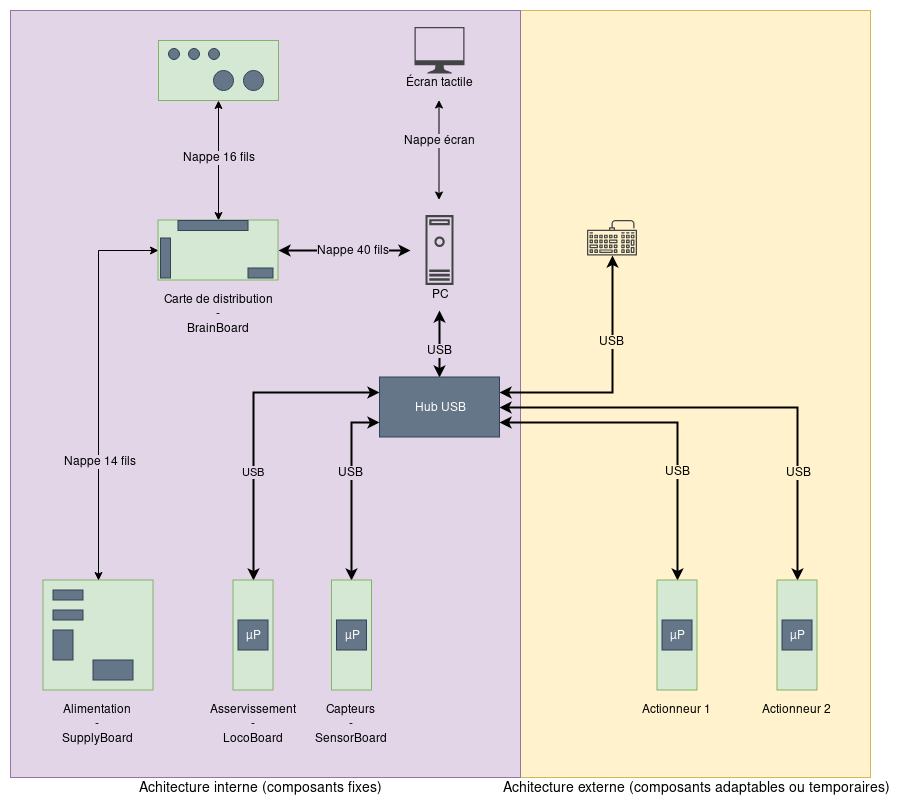
\includegraphics[width=1\textwidth]{pictures/arch_data}
	\end{figure}
	La communication est organisée selon une topologie en étoile, autour d'un
	Raspberry Pi 3B, servant de PC principal. Le PC fait tourner une IHM
	développée en C++, affichée sur l'écran Rasbperry Pi (ici l'écran officiel
	est utilisé pour des raisons de trésorerie et pour la garantie de se
	compatibilitée). L'écran est relié via sa nappe directement au PC. Son 
	alimentation est évoquée dans la section Architecture d'alimentation.



\subsection{Architecture d'alimentation}


\section{Alimentation}

\section{Asservissement}

\section{Contrôle}

%	\begin{figure}[h]
%		\caption{$Z_R$ en circuit ouvert et $Z_G = 50\Omega$}
%		\begin{subfigure}{.5\textwidth}
%			\centering
%			\includegraphics[width=0.9\textwidth]{QI-1}
%			\caption{Tension au point A}
%		\end{subfigure}%
%		\begin{subfigure}{.5\textwidth}
%			\centering
%			\includegraphics[width=0.9\textwidth]{QI-2}
%			\caption{Tension au point B}
%		\end{subfigure}
%	\end{figure}

\end{document}

